\section{Математические модели работы нейронов}
\subsection{Детерминистская модель}
\begin{figure}[h]
\center{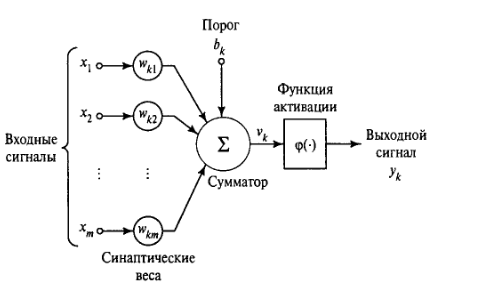
\includegraphics[width=0.8\linewidth]{BlockSheme.png}}
\caption{Явная нелинейная модель нейрона.}
\label{ris:BlockScheme}
\end{figure}
Как было выяснено ранее, нейрон представляет собой единицу обработки информации в нейронной сети. 
На блок-схеме рис.~\ref{ris:BlockScheme} показана модель нейрона, лежащая в основе искусственных нейронных сетей.
В этой модели можно выделить три основных функциональных элемента.
\begin{enumerate}
\item Набор синапсов или связей, каждый из которых характеризуется своим весом или силой.
В частности, сигнал $x_j$ на входе синапса $j$, связанного с нейроном $k$, умножается на вес $\omega_{jk}$.
В отличии от синапсов мозга синаптический вес искусственного может принимать как положительные, так и отрицательные значения. 
\item Сумматор складывает входные сигналы, взвешенные относительно соответствующих весов синапсов нейронов.
Математически эту операцию можно описать как линейную комбинацию входных сигналов.
\item Функция активации ограничивает выходную амплитуду сигнала нейрона.
Эта функция также называется функцией сжатия.
Обычно выходной сигнал нормализуется в диапазоне $[0;1]$ или $[-1;1]$.
\end{enumerate}
В модель нейрона, показанную на рис.~\ref{ris:BlockScheme}, включён пороговый элемент, который обозначается символом $b_k$.
Эта величина отражает увеличение или уменьшение входного сигнала функции активации.
В математической форме функционирование нейрона $k$ можно описать следующей парой уравнений:
\begin{equation}
u_k = \sum_{j=1}^{m} \omega_{kj}x_j
\end{equation}
\begin{equation}
y_k = \varphi (u_k + b_k)
\end{equation}
где $x_1,x_2,\dots,x_m$ --- входные сигналы;
$\omega_{k1},\omega_{k2},\dots,\omega_{km}$ --- синаптические веса нейрона $k$;
$u_k$ --- линейная комбинация входных воздействий;
$b_k$ --- порог;
$\varphi()$ --- функция активации;
$y_k$ --- выходной сигнал нейрона.\cite{NejronnyeSeti}
\subsection{Функции активации}
Функция активации, представленные в формулах как $\varphi()$, определяет выходной сигнал нейрона.
Можно выделить три основных типов функции активации.
\begin{enumerate}
\item Функция единичного скачка, или пороговая функция.
Этот тип функции описывается следующим уравнением:
\begin{equation}
\varphi(v) = 
\begin{cases}
1, v \ge 0\\
0, v < 0
\end{cases}
\end{equation}
В технической литературе эта форма функции единичного скачка называется функцией Хэвисайда.
Соответственно выходной сигнал нейрона $k$ можно представить как
\begin{equation}
y_k = 
\begin{cases}
1, v_k \ge 0\\
0, v_k < 0
\end{cases}
\end{equation}
где $v_k$ --- индуцированное локальное поле нейрона $k$.
Эту модель в литературе называют моделью Мак-Каллока-Питца. В этой модели выходной сигнал нейрона принимает значение 1 при неотрицательном индуцированном локальным полем, и 0 --- в противном случае.
Это выражение описывает свойство <<все или ничего>> модели Мак-Каллока-Питца.
\item Кусочно-линейная функция. Кусочно-линейная функция описывается следующим выражений:
\begin{equation}
\varphi(v) = 
\begin{cases}
1, v \ge +\frac12\\
|v|, -\frac12<v<+\frac12\\
0, v \le -\frac12
\end{cases}
\end{equation}
где коэффициент усиления в линейной области оператора предполагается равным единице.
Следующие два варианта можно считать особой формой кусочно-линейной функции.
\begin{itemize}
\item Если линейная область не достигает порога насыщения, они превращается в линейный сумматор 
\item Если коэффициент усиления линейной области стремиться к бесконечности, то кусочно-линейная функция выражается в пороговую.
\end{itemize}
\item Сигмоидальная функция. 
Сигмоидальная функция, график которой напоминает букву S, является наиболее распространённой функцией для построения искусственных нейронных сетей.
Это быстрорастущая функция, поддерживающая баланс между линейным и нелинейным поведением.
Примером сигмоидальной функции может служить логистическая функция, задаваемая выражением:
\begin{equation}
\varphi(v) = \frac1{1+e^{-av}}
\end{equation}
где $a$ --- параметр наклона сигмоидальной функции.
Изменяя этот параметр можно построить функции с различной крутизной.
При бесконечно большом параметре наклона функция вырождается в пороговую.
Если пороговая функция принимает только два значения (0 и 1), то сигмоидальная функция принимает бесконечное количество значений в диапазоне $[0;1]$.
При этом сигмоидальная функция является в отличии от пороговой дифференцируемая.\cite{NejronnyeSeti}
\end{enumerate}
\subsection{Стохастическая модель}
Модель нейрона, рассмотренная выше, является строго детерминистской.
Это значит, что преобразование входного сигнала в выходной точно определено для всех значений входного сигнала.
Однако в некоторых случаях предпочтительно использовать стохастические (вероятностные) нейросетевые модели.
В подобных моделях нейрон находится в одном из двух состояний (+1 и -1).
Решение о переключении нейрона из одного состояния в другое производится с учётом вероятности этого события.
Обозначим состояние нейрона символом $x$, а вероятность активации нейрона --- функцией $P(v)$, где $v$ --- локальное индуцированное поле нейрона.
Тогда
\begin{equation}
x=
\begin{cases}
+1, \text{с вероятностью } P(v),\\
-1, \text{с вероятностью } 1-P(v)
\end{cases}
\end{equation}
Вероятность $P(v)$ описывается сигмоидальной функцией следующего вида:
\begin{equation}
P(v) = \frac1{1 + e^{- v/T}}
\end{equation}
где $T$ --- это аналог температуры, используемый для управления уровнем шума, и таким образом, степенью неопределённости переключения.
При этом параметр $T$ не имеет отношения к физической температуре. \cite{NejronnyeSeti}
